\documentclass[10pt]{article}
\usepackage[margin=1cm, bottom=2cm]{geometry}
\usepackage{tikz}
\usepackage[urlcolor=blue, colorlinks=true]{hyperref}
\usepackage{longtable}
\usepackage{multirow}

\begin{document}

\title{Report\\Assignment 1: The Matrix Universe}
\author{Timur Usmanov, B23-ISE-01}
\maketitle

\section*{Introduction}
Find the complete source code and tests at \url{https://github.com/Error10556/IntroToAI1}.

\section{PEAS Description}

In this problem, the Actor has to find the smallest number of moves required to reach the destination cell.

\begin{enumerate}
	\item The Actor's performance measures, in order of priority, are:
	\begin{enumerate}
		\item The Actor survives;
		\item The Actor gives the correct answer;
		\item The Actor spends as few moves as possible until he can give an answer.
	\end{enumerate}
	
	\item The Actor's environment is a grid of $9\times 9$ cells, where each cell might contain an Agent, a Sentinel, the Backdoor key, or the Keymaker. This environment is:
	
	\begin{enumerate}
		\item \textbf{Partially observable}, because Neo only sees in a Moore neighborhood of range 1 or 2;
		\item \textbf{Multi-agent}, because, arguably, Agents and Sentinels have to observe their environment and kill Neo, which is an action;
		\item \textbf{Deterministic}, because there are no random elements; the environment is entirely predictable;
		\item \textbf{Sequential}, because the action of picking up the key changes the environment and would require Neo to make different moves;
		\item \textbf{Static}, because the environment does not change while the Actor thinks;
		\item \textbf{Discrete}, because there is only a finite number of states of the environment;
		\item \textbf{Known}, because the rules are given in the assignment.
	\end{enumerate}
	
	\item Neo's actuators are his legs (to make moves) and hands (to pick up the Backdoor key). Formally, the actuator is the \texttt{m x y} command.
	
	\item Neo's sensors are his eyes and the Trinity, which allow him to see the objects on the map and the perceived cells. Formally, our sensor is the standard input stream.
\end{enumerate}

\section{Algorithm flow}
\subsection{A*}
In this algorithm, each known cell is associated with several values: (a) the true shortest distance $d$ from $(0, 0)$ to that cell over safe cells, (b) the Manhattan distance $m$ from that cell to the Keymaker, (c) whether the cell is \textit{safe}, \textit{dangerous}, or \textit{unknown}, (d) whether or not the cell has been visited.
We define the estimate $E(c)$ of cell $c$ as $d + m$.

Neo first observes the surroundings at cell $(0, 0)$. Then, in a cycle, the Actor does the following:\newline
Neo chooses a safe cell $c$ that is adjacent to a previously visited cell, among those~--- with the least $E(c)$, among those~--- with the least $m$, among those~--- the one closest to Neo if he has to walk on safe cells to reach it (the distance is, again, calculated via another A* algorithm). Then, Neo moves there, scanning the surroundings and updating the map. Upon reaching the cell $c$, Neo updates the values associated with the adjacent unvisited cells of $c$. Once we have set the true shortest distance $d$ of the Keymaker cell, we may break out of the cycle. If there are no unvisited cells adjacent to a visited one, we know that there is no answer.

We ignore the Backdoor key, as it ``is not an obligation" ``to utilize its advantages".

\subsection{Backtracking}
In this algorithm, each cell is associated with the shortest distance from the start to this cell. An unexplored cell is marked with distance \texttt{-1}.

Neo explores the safe and reachable portion of the map using Depth-First Search (DFS). DFS assigns distances to cells upon reaching them and does not explore already visited cells that have been previously reached with fewer moves. Moreover, the Actor does not make a move if it guarantees a dead-end, or the number of moves is already exceeding the best known answer, or the theoretical best answer has already been found. When there are no adjacent suitable cells, Neo backtracks.

Again, we ignore the Backdoor key.

\section{Statistical analysis}
\subsection{Impossible tests}
A total of $1000$ tests were generated, out of which exactly 10 have no path to the Keymaker (if we ignore the Backdoor key).

\begin{center}
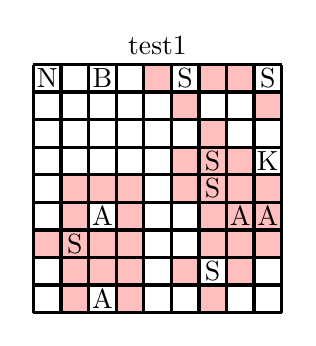
\begin{tikzpicture}[scale=0.35, baseline=0]\node[above] at (4.5,0) {test1};
    \node at (0.5,-0.5) {N};
    \fill[pink] (0,-6) rectangle (1,-7);
    \fill[pink] (1,-4) rectangle (2,-5);
    \fill[pink] (1,-5) rectangle (2,-6);
    \fill[pink] (1,-6) rectangle (2,-7);
    \node at (1.5,-6.5) {S};
    \fill[pink] (1,-7) rectangle (2,-8);
    \fill[pink] (1,-8) rectangle (2,-9);
    \node at (2.5,-0.5) {B};
    \fill[pink] (2,-4) rectangle (3,-5);
    \node at (2.5,-5.5) {A};
    \fill[pink] (2,-6) rectangle (3,-7);
    \fill[pink] (2,-7) rectangle (3,-8);
    \node at (2.5,-8.5) {A};
    \fill[pink] (3,-4) rectangle (4,-5);
    \fill[pink] (3,-5) rectangle (4,-6);
    \fill[pink] (3,-6) rectangle (4,-7);
    \fill[pink] (3,-7) rectangle (4,-8);
    \fill[pink] (3,-8) rectangle (4,-9);
    \fill[pink] (4,0) rectangle (5,-1);
    \node at (5.5,-0.5) {S};
    \fill[pink] (5,-1) rectangle (6,-2);
    \fill[pink] (5,-3) rectangle (6,-4);
    \fill[pink] (5,-4) rectangle (6,-5);
    \fill[pink] (5,-7) rectangle (6,-8);
    \fill[pink] (6,0) rectangle (7,-1);
    \fill[pink] (6,-2) rectangle (7,-3);
    \fill[pink] (6,-3) rectangle (7,-4);
    \node at (6.5,-3.5) {S};
    \fill[pink] (6,-4) rectangle (7,-5);
    \node at (6.5,-4.5) {S};
    \fill[pink] (6,-5) rectangle (7,-6);
    \fill[pink] (6,-6) rectangle (7,-7);
    \node at (6.5,-7.5) {S};
    \fill[pink] (6,-8) rectangle (7,-9);
    \fill[pink] (7,0) rectangle (8,-1);
    \fill[pink] (7,-3) rectangle (8,-4);
    \fill[pink] (7,-4) rectangle (8,-5);
    \fill[pink] (7,-5) rectangle (8,-6);
    \node at (7.5,-5.5) {A};
    \fill[pink] (7,-6) rectangle (8,-7);
    \fill[pink] (7,-7) rectangle (8,-8);
    \node at (8.5,-0.5) {S};
    \fill[pink] (8,-1) rectangle (9,-2);
    \node at (8.5,-3.5) {K};
    \fill[pink] (8,-4) rectangle (9,-5);
    \fill[pink] (8,-5) rectangle (9,-6);
    \node at (8.5,-5.5) {A};
    \fill[pink] (8,-6) rectangle (9,-7);
    \draw[very thick, step=1.0] (0,0) grid (9,-9);
\end{tikzpicture}
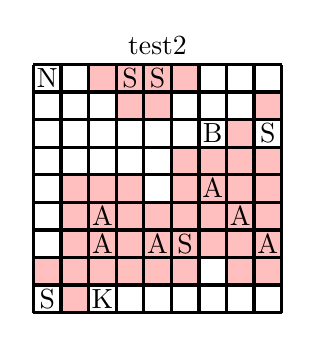
\begin{tikzpicture}[scale=0.35, baseline=0]\node[above] at (4.5,0) {test2};
    \node at (0.5,-0.5) {N};
    \fill[pink] (0,-7) rectangle (1,-8);
    \node at (0.5,-8.5) {S};
    \fill[pink] (1,-4) rectangle (2,-5);
    \fill[pink] (1,-5) rectangle (2,-6);
    \fill[pink] (1,-6) rectangle (2,-7);
    \fill[pink] (1,-7) rectangle (2,-8);
    \fill[pink] (1,-8) rectangle (2,-9);
    \fill[pink] (2,0) rectangle (3,-1);
    \fill[pink] (2,-4) rectangle (3,-5);
    \fill[pink] (2,-5) rectangle (3,-6);
    \node at (2.5,-5.5) {A};
    \fill[pink] (2,-6) rectangle (3,-7);
    \node at (2.5,-6.5) {A};
    \fill[pink] (2,-7) rectangle (3,-8);
    \node at (2.5,-8.5) {K};
    \fill[pink] (3,0) rectangle (4,-1);
    \node at (3.5,-0.5) {S};
    \fill[pink] (3,-1) rectangle (4,-2);
    \fill[pink] (3,-4) rectangle (4,-5);
    \fill[pink] (3,-5) rectangle (4,-6);
    \fill[pink] (3,-6) rectangle (4,-7);
    \fill[pink] (3,-7) rectangle (4,-8);
    \fill[pink] (4,0) rectangle (5,-1);
    \node at (4.5,-0.5) {S};
    \fill[pink] (4,-1) rectangle (5,-2);
    \fill[pink] (4,-5) rectangle (5,-6);
    \fill[pink] (4,-6) rectangle (5,-7);
    \node at (4.5,-6.5) {A};
    \fill[pink] (4,-7) rectangle (5,-8);
    \fill[pink] (5,0) rectangle (6,-1);
    \fill[pink] (5,-3) rectangle (6,-4);
    \fill[pink] (5,-4) rectangle (6,-5);
    \fill[pink] (5,-5) rectangle (6,-6);
    \fill[pink] (5,-6) rectangle (6,-7);
    \node at (5.5,-6.5) {S};
    \fill[pink] (5,-7) rectangle (6,-8);
    \node at (6.5,-2.5) {B};
    \fill[pink] (6,-3) rectangle (7,-4);
    \fill[pink] (6,-4) rectangle (7,-5);
    \node at (6.5,-4.5) {A};
    \fill[pink] (6,-5) rectangle (7,-6);
    \fill[pink] (6,-6) rectangle (7,-7);
    \fill[pink] (7,-2) rectangle (8,-3);
    \fill[pink] (7,-3) rectangle (8,-4);
    \fill[pink] (7,-4) rectangle (8,-5);
    \fill[pink] (7,-5) rectangle (8,-6);
    \node at (7.5,-5.5) {A};
    \fill[pink] (7,-6) rectangle (8,-7);
    \fill[pink] (7,-7) rectangle (8,-8);
    \fill[pink] (8,-1) rectangle (9,-2);
    \node at (8.5,-2.5) {S};
    \fill[pink] (8,-3) rectangle (9,-4);
    \fill[pink] (8,-4) rectangle (9,-5);
    \fill[pink] (8,-5) rectangle (9,-6);
    \fill[pink] (8,-6) rectangle (9,-7);
    \node at (8.5,-6.5) {A};
    \fill[pink] (8,-7) rectangle (9,-8);
    \draw[very thick, step=1.0] (0,0) grid (9,-9);
\end{tikzpicture}
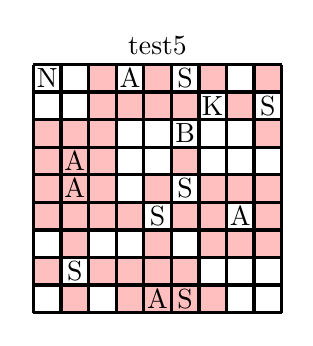
\begin{tikzpicture}[scale=0.35, baseline=0]\node[above] at (4.5,0) {test5};
    \node at (0.5,-0.5) {N};
    \fill[pink] (0,-2) rectangle (1,-3);
    \fill[pink] (0,-3) rectangle (1,-4);
    \fill[pink] (0,-4) rectangle (1,-5);
    \fill[pink] (0,-5) rectangle (1,-6);
    \fill[pink] (0,-7) rectangle (1,-8);
    \fill[pink] (1,-2) rectangle (2,-3);
    \fill[pink] (1,-3) rectangle (2,-4);
    \node at (1.5,-3.5) {A};
    \fill[pink] (1,-4) rectangle (2,-5);
    \node at (1.5,-4.5) {A};
    \fill[pink] (1,-5) rectangle (2,-6);
    \fill[pink] (1,-6) rectangle (2,-7);
    \node at (1.5,-7.5) {S};
    \fill[pink] (1,-8) rectangle (2,-9);
    \fill[pink] (2,0) rectangle (3,-1);
    \fill[pink] (2,-1) rectangle (3,-2);
    \fill[pink] (2,-2) rectangle (3,-3);
    \fill[pink] (2,-3) rectangle (3,-4);
    \fill[pink] (2,-4) rectangle (3,-5);
    \fill[pink] (2,-5) rectangle (3,-6);
    \fill[pink] (2,-7) rectangle (3,-8);
    \node at (3.5,-0.5) {A};
    \fill[pink] (3,-1) rectangle (4,-2);
    \fill[pink] (3,-5) rectangle (4,-6);
    \fill[pink] (3,-7) rectangle (4,-8);
    \fill[pink] (3,-8) rectangle (4,-9);
    \fill[pink] (4,0) rectangle (5,-1);
    \fill[pink] (4,-1) rectangle (5,-2);
    \fill[pink] (4,-4) rectangle (5,-5);
    \node at (4.5,-5.5) {S};
    \fill[pink] (4,-6) rectangle (5,-7);
    \fill[pink] (4,-7) rectangle (5,-8);
    \fill[pink] (4,-8) rectangle (5,-9);
    \node at (4.5,-8.5) {A};
    \node at (5.5,-0.5) {S};
    \fill[pink] (5,-1) rectangle (6,-2);
    \node at (5.5,-2.5) {B};
    \fill[pink] (5,-3) rectangle (6,-4);
    \node at (5.5,-4.5) {S};
    \fill[pink] (5,-5) rectangle (6,-6);
    \fill[pink] (5,-7) rectangle (6,-8);
    \fill[pink] (5,-8) rectangle (6,-9);
    \node at (5.5,-8.5) {S};
    \fill[pink] (6,0) rectangle (7,-1);
    \node at (6.5,-1.5) {K};
    \fill[pink] (6,-4) rectangle (7,-5);
    \fill[pink] (6,-5) rectangle (7,-6);
    \fill[pink] (6,-6) rectangle (7,-7);
    \fill[pink] (6,-8) rectangle (7,-9);
    \fill[pink] (7,-1) rectangle (8,-2);
    \fill[pink] (7,-4) rectangle (8,-5);
    \node at (7.5,-5.5) {A};
    \fill[pink] (7,-6) rectangle (8,-7);
    \fill[pink] (8,0) rectangle (9,-1);
    \node at (8.5,-1.5) {S};
    \fill[pink] (8,-2) rectangle (9,-3);
    \fill[pink] (8,-4) rectangle (9,-5);
    \fill[pink] (8,-5) rectangle (9,-6);
    \fill[pink] (8,-6) rectangle (9,-7);
    \draw[very thick, step=1.0] (0,0) grid (9,-9);
\end{tikzpicture}
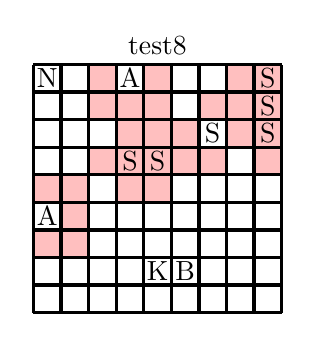
\begin{tikzpicture}[scale=0.35, baseline=0]\node[above] at (4.5,0) {test8};
    \node at (0.5,-0.5) {N};
    \fill[pink] (0,-4) rectangle (1,-5);
    \node at (0.5,-5.5) {A};
    \fill[pink] (0,-6) rectangle (1,-7);
    \fill[pink] (1,-4) rectangle (2,-5);
    \fill[pink] (1,-5) rectangle (2,-6);
    \fill[pink] (1,-6) rectangle (2,-7);
    \fill[pink] (2,0) rectangle (3,-1);
    \fill[pink] (2,-1) rectangle (3,-2);
    \fill[pink] (2,-3) rectangle (3,-4);
    \node at (3.5,-0.5) {A};
    \fill[pink] (3,-1) rectangle (4,-2);
    \fill[pink] (3,-2) rectangle (4,-3);
    \fill[pink] (3,-3) rectangle (4,-4);
    \node at (3.5,-3.5) {S};
    \fill[pink] (3,-4) rectangle (4,-5);
    \fill[pink] (4,0) rectangle (5,-1);
    \fill[pink] (4,-1) rectangle (5,-2);
    \fill[pink] (4,-2) rectangle (5,-3);
    \fill[pink] (4,-3) rectangle (5,-4);
    \node at (4.5,-3.5) {S};
    \fill[pink] (4,-4) rectangle (5,-5);
    \node at (4.5,-7.5) {K};
    \fill[pink] (5,-2) rectangle (6,-3);
    \fill[pink] (5,-3) rectangle (6,-4);
    \node at (5.5,-7.5) {B};
    \fill[pink] (6,-1) rectangle (7,-2);
    \node at (6.5,-2.5) {S};
    \fill[pink] (6,-3) rectangle (7,-4);
    \fill[pink] (7,0) rectangle (8,-1);
    \fill[pink] (7,-1) rectangle (8,-2);
    \fill[pink] (7,-2) rectangle (8,-3);
    \fill[pink] (8,0) rectangle (9,-1);
    \node at (8.5,-0.5) {S};
    \fill[pink] (8,-1) rectangle (9,-2);
    \node at (8.5,-1.5) {S};
    \fill[pink] (8,-2) rectangle (9,-3);
    \node at (8.5,-2.5) {S};
    \fill[pink] (8,-3) rectangle (9,-4);
    \draw[very thick, step=1.0] (0,0) grid (9,-9);
\end{tikzpicture}
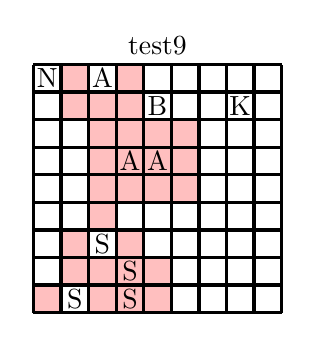
\begin{tikzpicture}[scale=0.35, baseline=0]\node[above] at (4.5,0) {test9};
    \node at (0.5,-0.5) {N};
    \fill[pink] (0,-8) rectangle (1,-9);
    \fill[pink] (1,0) rectangle (2,-1);
    \fill[pink] (1,-1) rectangle (2,-2);
    \fill[pink] (1,-6) rectangle (2,-7);
    \fill[pink] (1,-7) rectangle (2,-8);
    \node at (1.5,-8.5) {S};
    \node at (2.5,-0.5) {A};
    \fill[pink] (2,-1) rectangle (3,-2);
    \fill[pink] (2,-2) rectangle (3,-3);
    \fill[pink] (2,-3) rectangle (3,-4);
    \fill[pink] (2,-4) rectangle (3,-5);
    \fill[pink] (2,-5) rectangle (3,-6);
    \node at (2.5,-6.5) {S};
    \fill[pink] (2,-7) rectangle (3,-8);
    \fill[pink] (2,-8) rectangle (3,-9);
    \fill[pink] (3,0) rectangle (4,-1);
    \fill[pink] (3,-1) rectangle (4,-2);
    \fill[pink] (3,-2) rectangle (4,-3);
    \fill[pink] (3,-3) rectangle (4,-4);
    \node at (3.5,-3.5) {A};
    \fill[pink] (3,-4) rectangle (4,-5);
    \fill[pink] (3,-6) rectangle (4,-7);
    \fill[pink] (3,-7) rectangle (4,-8);
    \node at (3.5,-7.5) {S};
    \fill[pink] (3,-8) rectangle (4,-9);
    \node at (3.5,-8.5) {S};
    \node at (4.5,-1.5) {B};
    \fill[pink] (4,-2) rectangle (5,-3);
    \fill[pink] (4,-3) rectangle (5,-4);
    \node at (4.5,-3.5) {A};
    \fill[pink] (4,-4) rectangle (5,-5);
    \fill[pink] (4,-7) rectangle (5,-8);
    \fill[pink] (4,-8) rectangle (5,-9);
    \fill[pink] (5,-2) rectangle (6,-3);
    \fill[pink] (5,-3) rectangle (6,-4);
    \fill[pink] (5,-4) rectangle (6,-5);
    \node at (7.5,-1.5) {K};
    \draw[very thick, step=1.0] (0,0) grid (9,-9);
\end{tikzpicture}
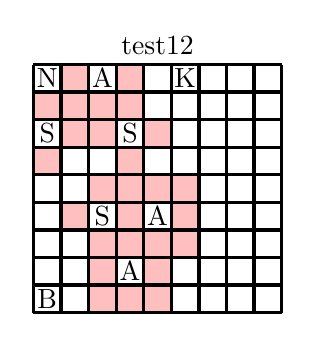
\begin{tikzpicture}[scale=0.35, baseline=0]\node[above] at (4.5,0) {test12};
\node at (0.5,-0.5) {N};
\fill[pink] (0,-1) rectangle (1,-2);
\node at (0.5,-2.5) {S};
\fill[pink] (0,-3) rectangle (1,-4);
\node at (0.5,-8.5) {B};
\fill[pink] (1,0) rectangle (2,-1);
\fill[pink] (1,-1) rectangle (2,-2);
\fill[pink] (1,-2) rectangle (2,-3);
\fill[pink] (1,-5) rectangle (2,-6);
\node at (2.5,-0.5) {A};
\fill[pink] (2,-1) rectangle (3,-2);
\fill[pink] (2,-2) rectangle (3,-3);
\fill[pink] (2,-4) rectangle (3,-5);
\node at (2.5,-5.5) {S};
\fill[pink] (2,-6) rectangle (3,-7);
\fill[pink] (2,-7) rectangle (3,-8);
\fill[pink] (2,-8) rectangle (3,-9);
\fill[pink] (3,0) rectangle (4,-1);
\fill[pink] (3,-1) rectangle (4,-2);
\node at (3.5,-2.5) {S};
\fill[pink] (3,-3) rectangle (4,-4);
\fill[pink] (3,-4) rectangle (4,-5);
\fill[pink] (3,-5) rectangle (4,-6);
\fill[pink] (3,-6) rectangle (4,-7);
\node at (3.5,-7.5) {A};
\fill[pink] (3,-8) rectangle (4,-9);
\fill[pink] (4,-2) rectangle (5,-3);
\fill[pink] (4,-4) rectangle (5,-5);
\node at (4.5,-5.5) {A};
\fill[pink] (4,-6) rectangle (5,-7);
\fill[pink] (4,-7) rectangle (5,-8);
\fill[pink] (4,-8) rectangle (5,-9);
\node at (5.5,-0.5) {K};
\fill[pink] (5,-4) rectangle (6,-5);
\fill[pink] (5,-5) rectangle (6,-6);
\fill[pink] (5,-6) rectangle (6,-7);
\draw[very thick, step=1.0] (0,0) grid (9,-9);
\end{tikzpicture}
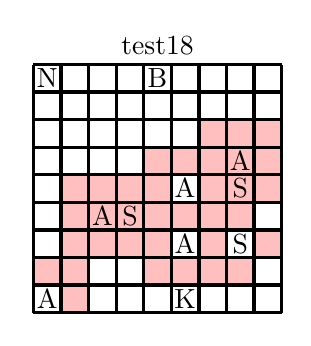
\begin{tikzpicture}[scale=0.35, baseline=0]\node[above] at (4.5,0) {test18};
\node at (0.5,-0.5) {N};
\fill[pink] (0,-7) rectangle (1,-8);
\node at (0.5,-8.5) {A};
\fill[pink] (1,-4) rectangle (2,-5);
\fill[pink] (1,-5) rectangle (2,-6);
\fill[pink] (1,-6) rectangle (2,-7);
\fill[pink] (1,-7) rectangle (2,-8);
\fill[pink] (1,-8) rectangle (2,-9);
\fill[pink] (2,-4) rectangle (3,-5);
\fill[pink] (2,-5) rectangle (3,-6);
\node at (2.5,-5.5) {A};
\fill[pink] (2,-6) rectangle (3,-7);
\fill[pink] (3,-4) rectangle (4,-5);
\fill[pink] (3,-5) rectangle (4,-6);
\node at (3.5,-5.5) {S};
\fill[pink] (3,-6) rectangle (4,-7);
\node at (4.5,-0.5) {B};
\fill[pink] (4,-3) rectangle (5,-4);
\fill[pink] (4,-4) rectangle (5,-5);
\fill[pink] (4,-5) rectangle (5,-6);
\fill[pink] (4,-6) rectangle (5,-7);
\fill[pink] (4,-7) rectangle (5,-8);
\fill[pink] (5,-3) rectangle (6,-4);
\node at (5.5,-4.5) {A};
\fill[pink] (5,-5) rectangle (6,-6);
\node at (5.5,-6.5) {A};
\fill[pink] (5,-7) rectangle (6,-8);
\node at (5.5,-8.5) {K};
\fill[pink] (6,-2) rectangle (7,-3);
\fill[pink] (6,-3) rectangle (7,-4);
\fill[pink] (6,-4) rectangle (7,-5);
\fill[pink] (6,-5) rectangle (7,-6);
\fill[pink] (6,-6) rectangle (7,-7);
\fill[pink] (6,-7) rectangle (7,-8);
\fill[pink] (7,-2) rectangle (8,-3);
\fill[pink] (7,-3) rectangle (8,-4);
\node at (7.5,-3.5) {A};
\fill[pink] (7,-4) rectangle (8,-5);
\node at (7.5,-4.5) {S};
\fill[pink] (7,-5) rectangle (8,-6);
\node at (7.5,-6.5) {S};
\fill[pink] (7,-7) rectangle (8,-8);
\fill[pink] (8,-2) rectangle (9,-3);
\fill[pink] (8,-3) rectangle (9,-4);
\fill[pink] (8,-4) rectangle (9,-5);
\fill[pink] (8,-6) rectangle (9,-7);
\draw[very thick, step=1.0] (0,0) grid (9,-9);
\end{tikzpicture}
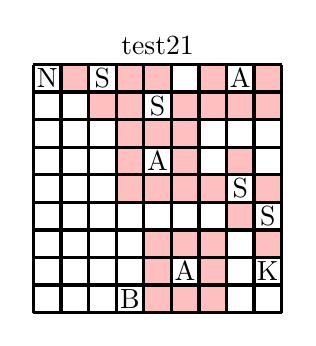
\begin{tikzpicture}[scale=0.35, baseline=0]\node[above] at (4.5,0) {test21};
    \node at (0.5,-0.5) {N};
    \fill[pink] (1,0) rectangle (2,-1);
    \node at (2.5,-0.5) {S};
    \fill[pink] (2,-1) rectangle (3,-2);
    \fill[pink] (3,0) rectangle (4,-1);
    \fill[pink] (3,-1) rectangle (4,-2);
    \fill[pink] (3,-2) rectangle (4,-3);
    \fill[pink] (3,-3) rectangle (4,-4);
    \fill[pink] (3,-4) rectangle (4,-5);
    \node at (3.5,-8.5) {B};
    \fill[pink] (4,0) rectangle (5,-1);
    \node at (4.5,-1.5) {S};
    \fill[pink] (4,-2) rectangle (5,-3);
    \node at (4.5,-3.5) {A};
    \fill[pink] (4,-4) rectangle (5,-5);
    \fill[pink] (4,-6) rectangle (5,-7);
    \fill[pink] (4,-7) rectangle (5,-8);
    \fill[pink] (4,-8) rectangle (5,-9);
    \fill[pink] (5,-1) rectangle (6,-2);
    \fill[pink] (5,-2) rectangle (6,-3);
    \fill[pink] (5,-3) rectangle (6,-4);
    \fill[pink] (5,-4) rectangle (6,-5);
    \fill[pink] (5,-6) rectangle (6,-7);
    \node at (5.5,-7.5) {A};
    \fill[pink] (5,-8) rectangle (6,-9);
    \fill[pink] (6,0) rectangle (7,-1);
    \fill[pink] (6,-1) rectangle (7,-2);
    \fill[pink] (6,-4) rectangle (7,-5);
    \fill[pink] (6,-6) rectangle (7,-7);
    \fill[pink] (6,-7) rectangle (7,-8);
    \fill[pink] (6,-8) rectangle (7,-9);
    \node at (7.5,-0.5) {A};
    \fill[pink] (7,-1) rectangle (8,-2);
    \fill[pink] (7,-3) rectangle (8,-4);
    \node at (7.5,-4.5) {S};
    \fill[pink] (7,-5) rectangle (8,-6);
    \fill[pink] (8,0) rectangle (9,-1);
    \fill[pink] (8,-1) rectangle (9,-2);
    \fill[pink] (8,-4) rectangle (9,-5);
    \node at (8.5,-5.5) {S};
    \fill[pink] (8,-6) rectangle (9,-7);
    \node at (8.5,-7.5) {K};
    \draw[very thick, step=1.0] (0,0) grid (9,-9);
\end{tikzpicture}
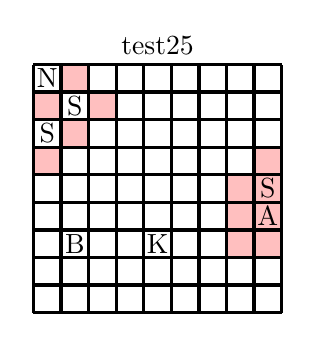
\begin{tikzpicture}[scale=0.35, baseline=0]\node[above] at (4.5,0) {test25};
    \node at (0.5,-0.5) {N};
    \fill[pink] (0,-1) rectangle (1,-2);
    \node at (0.5,-2.5) {S};
    \fill[pink] (0,-3) rectangle (1,-4);
    \fill[pink] (1,0) rectangle (2,-1);
    \node at (1.5,-1.5) {S};
    \fill[pink] (1,-2) rectangle (2,-3);
    \node at (1.5,-6.5) {B};
    \fill[pink] (2,-1) rectangle (3,-2);
    \node at (4.5,-6.5) {K};
    \fill[pink] (7,-4) rectangle (8,-5);
    \fill[pink] (7,-5) rectangle (8,-6);
    \fill[pink] (7,-6) rectangle (8,-7);
    \fill[pink] (8,-3) rectangle (9,-4);
    \fill[pink] (8,-4) rectangle (9,-5);
    \node at (8.5,-4.5) {S};
    \fill[pink] (8,-5) rectangle (9,-6);
    \node at (8.5,-5.5) {A};
    \fill[pink] (8,-6) rectangle (9,-7);
    \draw[very thick, step=1.0] (0,0) grid (9,-9);
\end{tikzpicture}
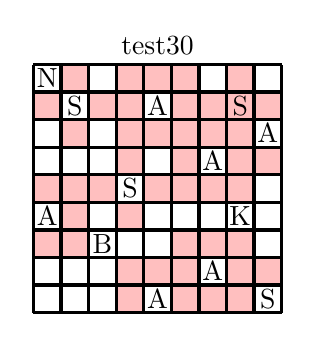
\begin{tikzpicture}[scale=0.35, baseline=0]\node[above] at (4.5,0) {test30};
    \node at (0.5,-0.5) {N};
    \fill[pink] (0,-1) rectangle (1,-2);
    \fill[pink] (0,-4) rectangle (1,-5);
    \node at (0.5,-5.5) {A};
    \fill[pink] (0,-6) rectangle (1,-7);
    \fill[pink] (1,0) rectangle (2,-1);
    \node at (1.5,-1.5) {S};
    \fill[pink] (1,-2) rectangle (2,-3);
    \fill[pink] (1,-4) rectangle (2,-5);
    \fill[pink] (1,-5) rectangle (2,-6);
    \fill[pink] (1,-6) rectangle (2,-7);
    \fill[pink] (2,-1) rectangle (3,-2);
    \fill[pink] (2,-4) rectangle (3,-5);
    \node at (2.5,-6.5) {B};
    \fill[pink] (3,0) rectangle (4,-1);
    \fill[pink] (3,-1) rectangle (4,-2);
    \fill[pink] (3,-2) rectangle (4,-3);
    \fill[pink] (3,-3) rectangle (4,-4);
    \node at (3.5,-4.5) {S};
    \fill[pink] (3,-5) rectangle (4,-6);
    \fill[pink] (3,-7) rectangle (4,-8);
    \fill[pink] (3,-8) rectangle (4,-9);
    \fill[pink] (4,0) rectangle (5,-1);
    \node at (4.5,-1.5) {A};
    \fill[pink] (4,-2) rectangle (5,-3);
    \fill[pink] (4,-4) rectangle (5,-5);
    \fill[pink] (4,-7) rectangle (5,-8);
    \node at (4.5,-8.5) {A};
    \fill[pink] (5,0) rectangle (6,-1);
    \fill[pink] (5,-1) rectangle (6,-2);
    \fill[pink] (5,-2) rectangle (6,-3);
    \fill[pink] (5,-3) rectangle (6,-4);
    \fill[pink] (5,-4) rectangle (6,-5);
    \fill[pink] (5,-6) rectangle (6,-7);
    \fill[pink] (5,-7) rectangle (6,-8);
    \fill[pink] (5,-8) rectangle (6,-9);
    \fill[pink] (6,-1) rectangle (7,-2);
    \fill[pink] (6,-2) rectangle (7,-3);
    \node at (6.5,-3.5) {A};
    \fill[pink] (6,-4) rectangle (7,-5);
    \fill[pink] (6,-6) rectangle (7,-7);
    \node at (6.5,-7.5) {A};
    \fill[pink] (6,-8) rectangle (7,-9);
    \fill[pink] (7,0) rectangle (8,-1);
    \fill[pink] (7,-1) rectangle (8,-2);
    \node at (7.5,-1.5) {S};
    \fill[pink] (7,-2) rectangle (8,-3);
    \fill[pink] (7,-3) rectangle (8,-4);
    \fill[pink] (7,-4) rectangle (8,-5);
    \node at (7.5,-5.5) {K};
    \fill[pink] (7,-6) rectangle (8,-7);
    \fill[pink] (7,-7) rectangle (8,-8);
    \fill[pink] (7,-8) rectangle (8,-9);
    \fill[pink] (8,-1) rectangle (9,-2);
    \node at (8.5,-2.5) {A};
    \fill[pink] (8,-3) rectangle (9,-4);
    \fill[pink] (8,-7) rectangle (9,-8);
    \node at (8.5,-8.5) {S};
    \draw[very thick, step=1.0] (0,0) grid (9,-9);
\end{tikzpicture}

\end{center}
\begin{flushright}
\textit{Legend:} \textbf{N}~--- Neo, \textbf{A}~--- Agent, \textbf{S}~--- Sentinel, \textbf{B}~--- Backdoor key, \textbf{K}~--- Keymaker, \tikz[baseline=0.1]{\fill[pink] (0,0) rectangle (0.3,0.3)}~--- a perceived cell.
\end{flushright}
\begin{figure}[!h]
\caption{Maps with the answer \texttt{-1}.}\label{impossibletests}
\end{figure}

\subsection{Algorithm comparison}
In Table \ref{comparison}, a ``win'' is defined as a situation where Neo can reach the Keymaker and the program can correctly determine the shortest distance to the goal.

\pagebreak

\begin{longtable}[c]{|c|c|c|c|c|c|}
	\hline
	\multicolumn{2}{|c|}{} & \textbf{A* (variant 1)} & \textbf{A* (variant 2)} & \textbf{Backtracking (v. 1)} & \textbf{Backtracking (v. 2)}\\
	\hline
	\endhead
	\multirow{4}{3cm}{Execution time, $\mu s$} & Mean & 1243.06 & 1259.61 & 28100.18 & 30429.94 \\\cline{2-6}
	& Mode & 1280 (7 times) & 1088 (6 times) & 1165 (3 times) & 1079 (2 times) \\\cline{2-6}
	& Median & 1201 & 1214.5 & 5561.5 & 5998 \\\cline{2-6}
	& SD & 223.19 & 241.83 & 82184.89 & 88253.63 \\\hline
	\multirow{4}{3cm}{Number of moves} & Mean & 11.35 & 11.35 & 1650.51 & 1650.49 \\\cline{2-6}
	& Mode & 9 (88 times) & 9 (88 times) & 11 (21 times) & 3 (21 times) \\\cline{2-6}
	& Median & 8 & 8 & 266 & 266 \\\cline{2-6}
	& SD & 10.73 & 10.73 & 5022.03 & 5022.03 \\\hline
	\multicolumn{2}{|c|}{Number of wins} & 990 (99\%) & 990 (99\%) & 990 (99\%) & 990 (99\%) \\\hline
	\multicolumn{2}{|c|}{Number of losses} & 10 (1\%) & 10 (1\%)  & 10 (1\%) & 10 (1\%) \\\hline
	\multicolumn{2}{|c|}{Executions longer than 1 sec} & 0 (0\%) & 0 (0\%) & 1 (0.1\%) & 1 (0.1\%)\\\hline
	
\end{longtable}

\setcounter{table}{0}

\begin{table}[!h]
	\caption{Statistics of algorithms side-by-side.} \label{comparison}
\end{table}

\subsection{Discussion}
The A* algorithm performs the same in both variants. Table \ref{comparison} shows a great similarity in each statistic of the two variants. However, the actual runtime of the program slightly increases as the field of view widens, although that may be a statistically insignificant increase. We conclude that the variant of the problem has no effect on the optimality of decisions of the Actor, but it probably slows down Neo's perception.

The Backtracking algorithm, however, suffers from the slow-down of the large perception area. The mean runtime of the program increases by 2 ms if the second variant of the problem is being solved. This fact could be explained by the large number of moves the algorithm makes (compared to A*). However, in rare cases, the algorithm makes fewer moves when given an increased range of perception. Overall, the Backtracking algorithm can take advantage of the large field of view in terms of the number of queries, but needs more resources to do so.

The Backtracking algorithm is totally inefficient in the worst cases. This is proven by the fact that the algorithm takes more than one second to solve test \#800 (see Fig. \ref{test800}).

\begin{figure}[!h]
\begin{center}
	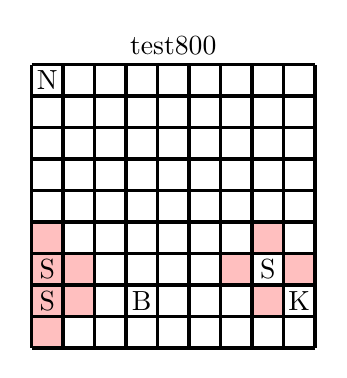
\begin{tikzpicture}[scale=0.4][baseline=0]
		\node[above] at (4.5,0) {test800};
		\node at (0.5,-0.5) {N};
		\fill[pink] (0,-5) rectangle (1,-6);
		\fill[pink] (0,-6) rectangle (1,-7);
		\node at (0.5,-6.5) {S};
		\fill[pink] (0,-7) rectangle (1,-8);
		\node at (0.5,-7.5) {S};
		\fill[pink] (0,-8) rectangle (1,-9);
		\fill[pink] (1,-6) rectangle (2,-7);
		\fill[pink] (1,-7) rectangle (2,-8);
		\node at (3.5,-7.5) {B};
		\fill[pink] (6,-6) rectangle (7,-7);
		\fill[pink] (7,-5) rectangle (8,-6);
		\node at (7.5,-6.5) {S};
		\fill[pink] (7,-7) rectangle (8,-8);
		\fill[pink] (8,-6) rectangle (9,-7);
		\node at (8.5,-7.5) {K};
		\draw[very thick, step=1.0] (0,0) grid (9,-9);
	\end{tikzpicture}
\end{center}
\caption{The worst case out of 1000 for backtracking} \label{test800}
\end{figure}

Clearly, A* beats Backtracking in every way except for correctness. The runtime is consistently shorter, and the number of moves is less by several orders of magnitude. While Backtracking outputs the same answers, A* does it much faster and is arguably not more difficult to implement. Moreover, since the efficiency of Backtracking solely depends on the applicability of certain heuristics (which are not always applicable), A* does not; therefore, A* has the advantage of being consistently performant.

\end{document}